\documentclass[12pt]{report}
\usepackage{amsmath}
\usepackage{geometry}

\usepackage{graphicx}

\title{Input/Outport Port}
\author{Amarjeet Singh Kapoor}
\begin{document}
\thispagestyle{plain}
	\begin{titlepage}
\maketitle
	\end{titlepage}
\section{Input/Output port}
 I/O port are basically interface needed for communication between processor and I/O device.
These are of two types:-
\begin{enumerate}
\item Non programmable
\item  programmable
\end{enumerate}

\section{Non-programmable I/O port}
These are fixed port which work either as input or output port only and there function cannot be changed and its example is Intel 8212


\section{Programmable I/O port}
Programmable I/O port is a multi port device which can be programmed to work in variety of ways as user likes. e.g. Intel 8255   

\section{Intel 8255} 
The Intel 8255 Programmable Peripheral Interface (PPI) chip is a peripheral chip originally developed for Intel 8085 microprocessor.It contains Three programmable port Ports Port A, Port B, Port C. 


The port C can be further divided into two ports of 4-bits each :- 
	 Port $C_{{UPPER}}$ Port $C_{{LOWER}}$

The 8255 operates in three modes -:
\begin{enumerate}
\item {Mode 0 -: all operate as simple I/O port }
\item {Mode 1 -: Port A,B operate as strobed I/O Port and Port C 
				act as control word.}
\item	{Mode 2 -: Port A operates as strobed bi-directional Port } \end{enumerate}
		 
\begin{figure}[!h]
	\centering
	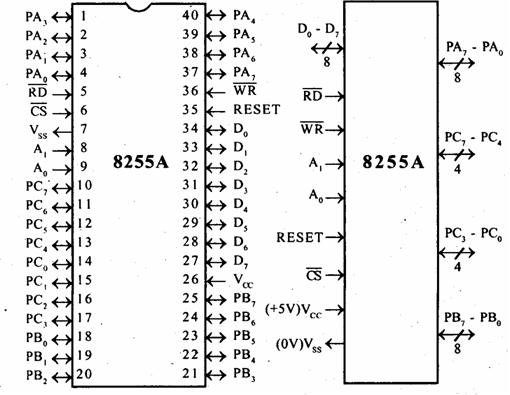
\includegraphics[scale=0.5]{0.png}
	  \caption{block diagram of Intel 8255}
\end{figure}

Programmer make use of control word that defines which 
port will act as an input or output.


\section{Serial Data Transfer}

Serial data transfer refers to the transfer of only one bit at a time. This is done for cost efficiency. Serial data can be transmitted in two modes:
\begin{enumerate}
\item {Asynchronous Mode}
\item  {Synchronous Mode}
\end{enumerate}

\subsection{Asynchronous Mode}

\begin{itemize}
\item{Transmission occurs at any time }
\item{Usually used for low speed transmission}
\item{Start bit is send at starting of transmission of data and end bits at end of transmission}
\end{itemize}

\subsection{synchronous Mode}

\begin{itemize}
\item{The transmitter and recevier are synchronized}
\item{Usually used for high speed transmission}
\item{Synchronization occure at beginning of long message}
\end{itemize}

\section{USART}
 
USART stands for Universal Asynchronous Synchronous Receiver- Transmitter. It is an IC used to convert serial data into parallel data so that the computer can process it and vice-versa. It also has an acknowledgement mechanism to make sure that the sender does not transmit at a rate higher than the receiver can handle.

\section{Intel 8251A} 
The 8251A is a programmable communication interface for serial data transmission. Its a type of USART. It accepts data in parallel format from the CPU and converts them into a continuous serial stream for transmission. Simultaneously, it can receive serial data streams and converts them into parallel data. The data so converted into parallel format are sent to the CPU for processing.



Types Of Control Words-:

1. mode word
2. command word
3. status word 

Before starting data transmission, control words are loaded into Intel 8251 


\subsection{Steps For Sending Data To CPU -:}
\begin{enumerate}
	\item TX RDY is connected to interrupt pin
	\item When TX RDY is high it can accept data
	\item When data is received it goes low
	\item Then data is converted in serial form through TXD line
	\item Rate of data is controlled by TXC pin
\end{enumerate}


\subsection{Steps For Receiving Data From I/O device-:}
\begin{enumerate}
\item when RX RDY is low it can accept data
\item when data is received it goes high
\item Then data is converted in parallel form through RXD line
\item Rate of data is controlled by RXC pin
\end{enumerate}

\begin{figure}[!h]
	\centering
	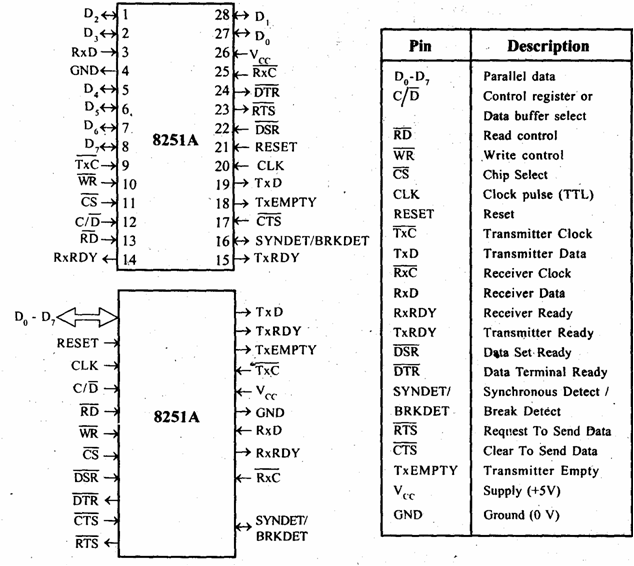
\includegraphics[scale=0.5]{5.png}
	  \caption{Block Diagram of Intel 8521 }
\end{figure}
\end{document}
